\documentclass[11pt,a4paper]{article}
\usepackage[utf8]{inputenc}
\usepackage[T1]{fontenc}
\usepackage{geometry}
\usepackage{tikz}
\usepackage{pgfplots}
\usepackage{amsmath}
\usepackage{amsfonts}
\usepackage{amssymb}
\usepackage{graphicx}
\usepackage{xcolor}
\usepackage{listings}
\usepackage{hyperref}
\usepackage{fancyhdr}
\usepackage{tcolorbox}
\usepackage{enumitem}
\usepackage{float}
\usepackage{subcaption}
\usepackage{algorithm}
\usepackage{algpseudocode}

% Page setup
\geometry{margin=1in}
\pagestyle{fancy}
\fancyhf{}
\rhead{LLM Detective - System Workflow}
\lhead{IIT Gandhinagar}
\cfoot{\thepage}

% TikZ libraries
\usetikzlibrary{shapes.geometric, arrows, positioning, fit, backgrounds, calc}

% Define colors
\definecolor{primaryblue}{RGB}{33, 150, 243}
\definecolor{secondarygreen}{RGB}{76, 175, 80}
\definecolor{accentorange}{RGB}{255, 152, 0}
\definecolor{dangerred}{RGB}{244, 67, 54}
\definecolor{warningyellow}{RGB}{255, 193, 7}
\definecolor{lightgray}{RGB}{245, 245, 245}
\definecolor{darkgray}{RGB}{66, 66, 66}

% TikZ styles
\tikzstyle{process} = [rectangle, rounded corners, minimum width=3cm, minimum height=1cm, text centered, draw=black, fill=primaryblue!20]
\tikzstyle{decision} = [diamond, minimum width=3cm, minimum height=1cm, text centered, draw=black, fill=warningyellow!30]
\tikzstyle{io} = [trapezium, trapezium left angle=70, trapezium right angle=110, minimum width=3cm, minimum height=1cm, text centered, draw=black, fill=secondarygreen!20]
\tikzstyle{storage} = [cylinder, shape border rotate=90, minimum width=2.5cm, minimum height=1.2cm, text centered, draw=black, fill=accentorange!20]
\tikzstyle{arrow} = [thick,->,>=stealth]
\tikzstyle{connector} = [circle, minimum width=0.8cm, text centered, draw=black, fill=lightgray]

% Custom commands
\newcommand{\systemname}{LLM Detective}
\newcommand{\subtitle}{AI-Powered Document Analysis System}

\title{
\Huge \textbf{\systemname} \\
\Large \subtitle \\
\vspace{0.5cm}
\large System Architecture \& Workflow Documentation
}
\author{
Vivek Raj \\
Indian Institute of Technology Gandhinagar \\
\texttt{vivek.raj@iitgn.ac.in}
}
\date{\today}

\begin{document}

\maketitle

\begin{abstract}
This document presents a comprehensive workflow analysis of the LLM Detective system, an advanced AI-powered document analysis platform designed to detect AI-generated content in PDF documents. The system combines optical character recognition (OCR), machine learning classification, and real-time web technologies to provide intelligent content analysis with visual feedback. This workflow documentation covers the complete system architecture, data flow, processing pipeline, and user interaction patterns.
\end{abstract}

\tableofcontents
\newpage

\section{System Overview}

\subsection{Introduction}
The \systemname{} is a sophisticated document analysis platform that leverages cutting-edge technologies to identify AI-generated content within PDF documents. The system employs a multi-tiered architecture combining FastAPI backend services, React frontend interfaces, and specialized machine learning models to deliver real-time analysis capabilities.

\subsection{Key Components}
\begin{itemize}
    \item \textbf{Frontend Interface}: React 19 with TypeScript and Material-UI
    \item \textbf{Backend API}: FastAPI with WebSocket support
    \item \textbf{OCR Engine}: Tesseract with PDF processing capabilities
    \item \textbf{ML Classification}: PyTorch-based transformer model
    \item \textbf{Authentication}: Firebase with IITGN email validation
    \item \textbf{Monitoring}: OpenTelemetry distributed tracing
\end{itemize}

\section{System Architecture}

\begin{figure}[H]
\centering
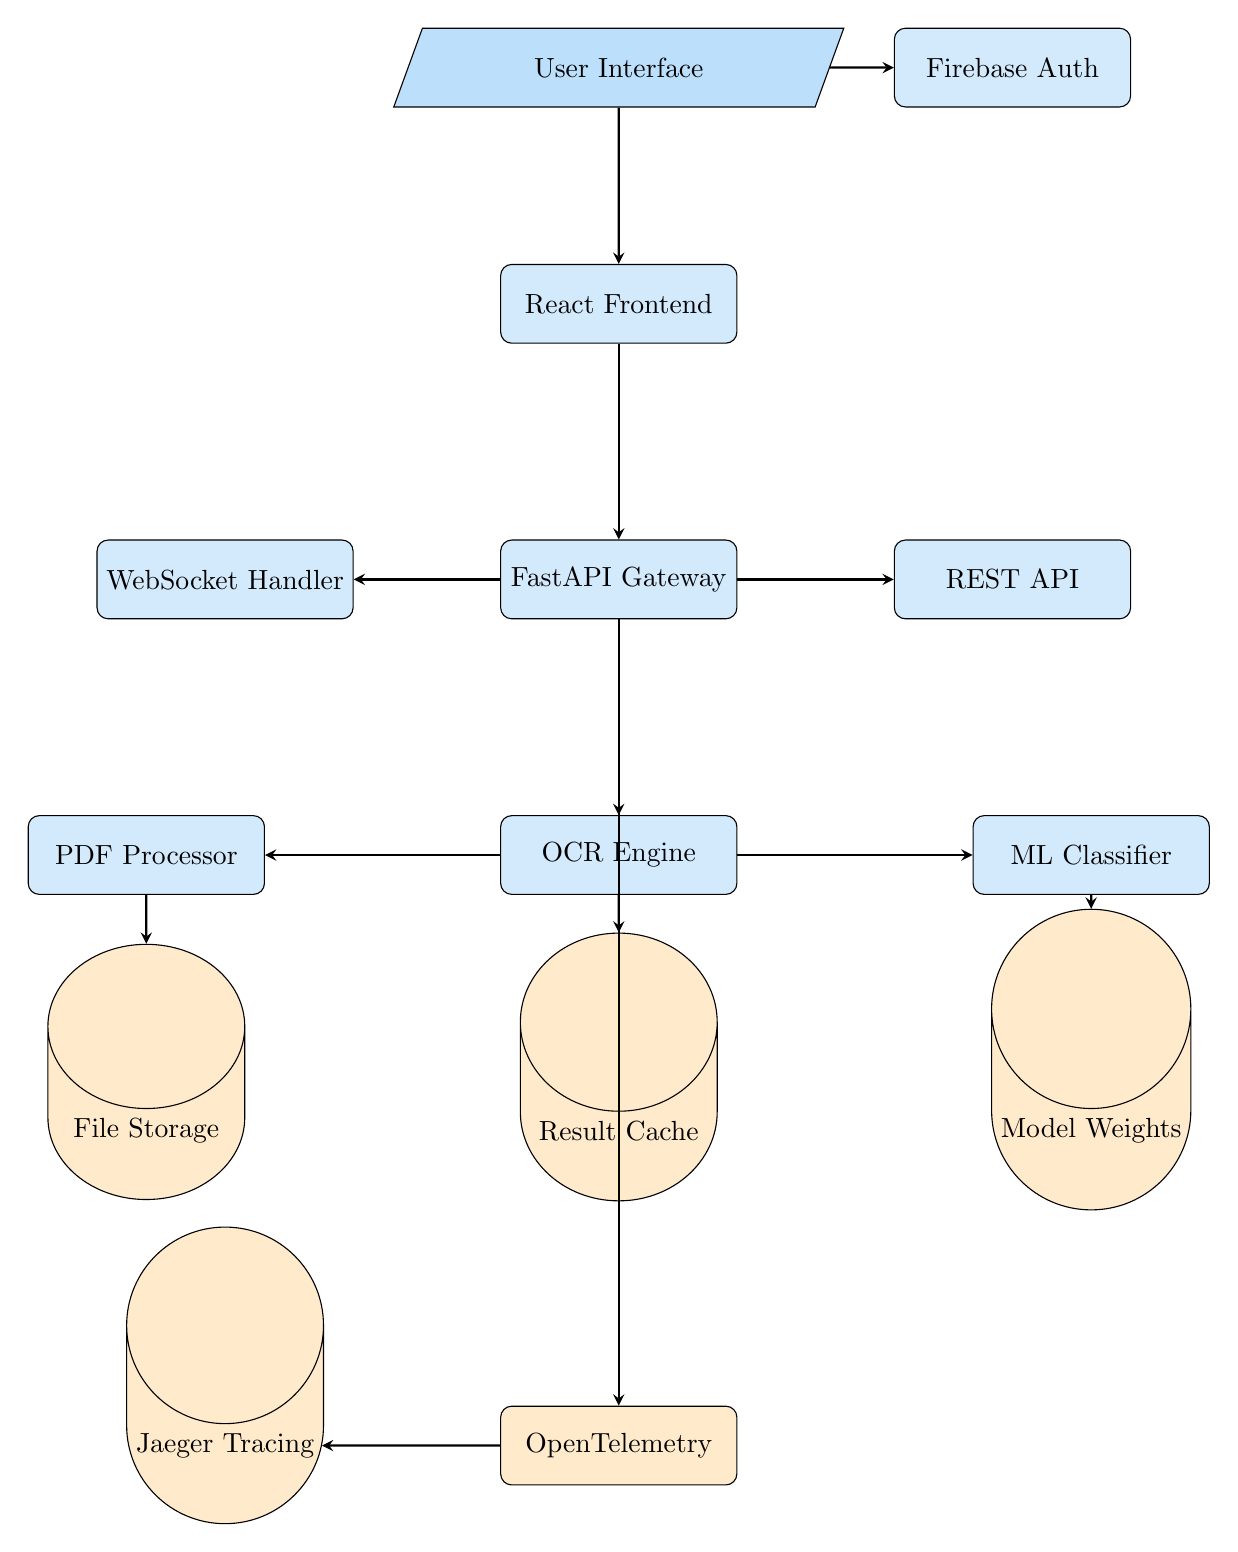
\begin{tikzpicture}[node distance=2cm]

% User Interface Layer
\node (user) [io, fill=primaryblue!30] {User Interface};
\node (auth) [process, right of=user, xshift=3cm] {Firebase Auth};
\node (frontend) [process, below of=user, yshift=-1cm] {React Frontend};

% API Gateway Layer
\node (api) [process, below of=frontend, yshift=-1.5cm] {FastAPI Gateway};
\node (websocket) [process, left of=api, xshift=-3cm] {WebSocket Handler};
\node (rest) [process, right of=api, xshift=3cm] {REST API};

% Processing Layer
\node (ocr) [process, below of=api, yshift=-1.5cm] {OCR Engine};
\node (ml) [process, right of=ocr, xshift=4cm] {ML Classifier};
\node (pdf) [process, left of=ocr, xshift=-4cm] {PDF Processor};

% Storage Layer
\node (uploads) [storage, below of=pdf, yshift=-1.5cm] {File Storage};
\node (model) [storage, below of=ml, yshift=-1.5cm] {Model Weights};
\node (cache) [storage, below of=ocr, yshift=-1.5cm] {Result Cache};

% Monitoring Layer
\node (telemetry) [process, below of=cache, yshift=-2cm, fill=accentorange!20] {OpenTelemetry};
\node (jaeger) [storage, left of=telemetry, xshift=-3cm, fill=accentorange!20] {Jaeger Tracing};

% Arrows
\draw [arrow] (user) -- (auth);
\draw [arrow] (user) -- (frontend);
\draw [arrow] (frontend) -- (api);
\draw [arrow] (api) -- (websocket);
\draw [arrow] (api) -- (rest);
\draw [arrow] (api) -- (ocr);
\draw [arrow] (ocr) -- (pdf);
\draw [arrow] (ocr) -- (ml);
\draw [arrow] (pdf) -- (uploads);
\draw [arrow] (ml) -- (model);
\draw [arrow] (ocr) -- (cache);
\draw [arrow] (api) -- (telemetry);
\draw [arrow] (telemetry) -- (jaeger);

\end{tikzpicture}
\caption{High-Level System Architecture}
\label{fig:architecture}
\end{figure}

\section{Detailed Workflow Process}

\subsection{User Authentication Flow}

\begin{figure}[H]
\centering
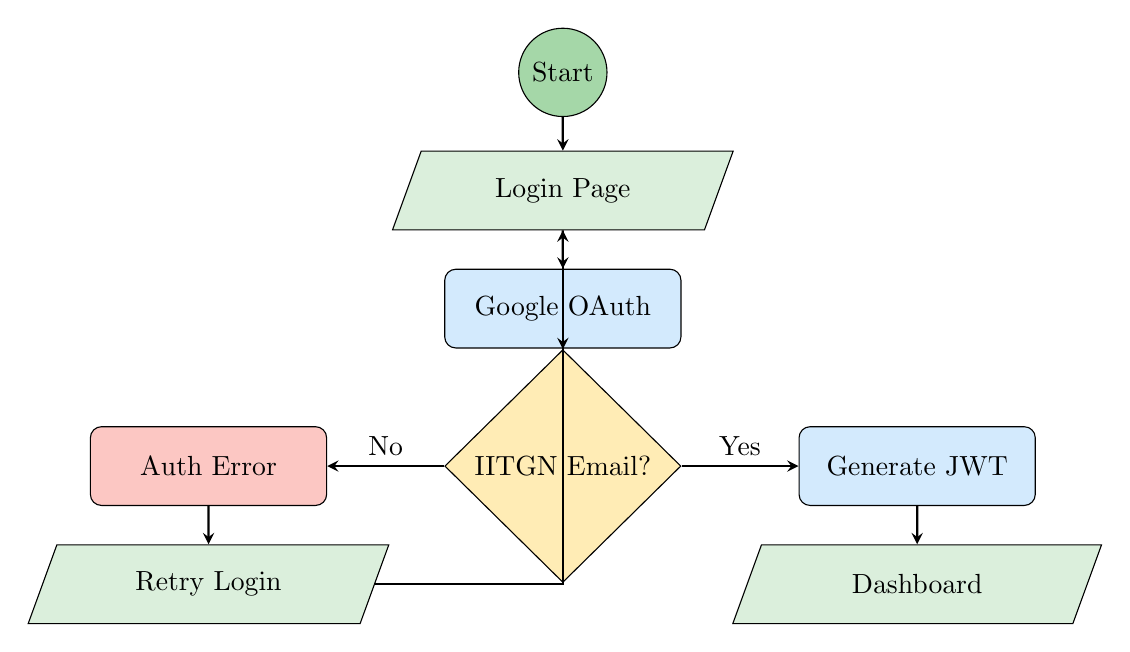
\begin{tikzpicture}[node distance=1.5cm]

\node (start) [connector, fill=secondarygreen!50] {Start};
\node (login) [io, below of=start] {Login Page};
\node (google) [process, below of=login] {Google OAuth};
\node (validate) [decision, below of=google, yshift=-0.5cm] {IITGN Email?};
\node (success) [process, right of=validate, xshift=3cm] {Generate JWT};
\node (dashboard) [io, below of=success] {Dashboard};
\node (error) [process, left of=validate, xshift=-3cm, fill=dangerred!30] {Auth Error};
\node (retry) [io, below of=error] {Retry Login};

% Arrows
\draw [arrow] (start) -- (login);
\draw [arrow] (login) -- (google);
\draw [arrow] (google) -- (validate);
\draw [arrow] (validate) -- node[anchor=south] {Yes} (success);
\draw [arrow] (validate) -- node[anchor=south] {No} (error);
\draw [arrow] (success) -- (dashboard);
\draw [arrow] (error) -- (retry);
\draw [arrow] (retry) -| (login);

\end{tikzpicture}
\caption{Authentication Workflow}
\label{fig:auth-flow}
\end{figure}

\subsection{Document Processing Pipeline}

\begin{figure}[H]
\centering
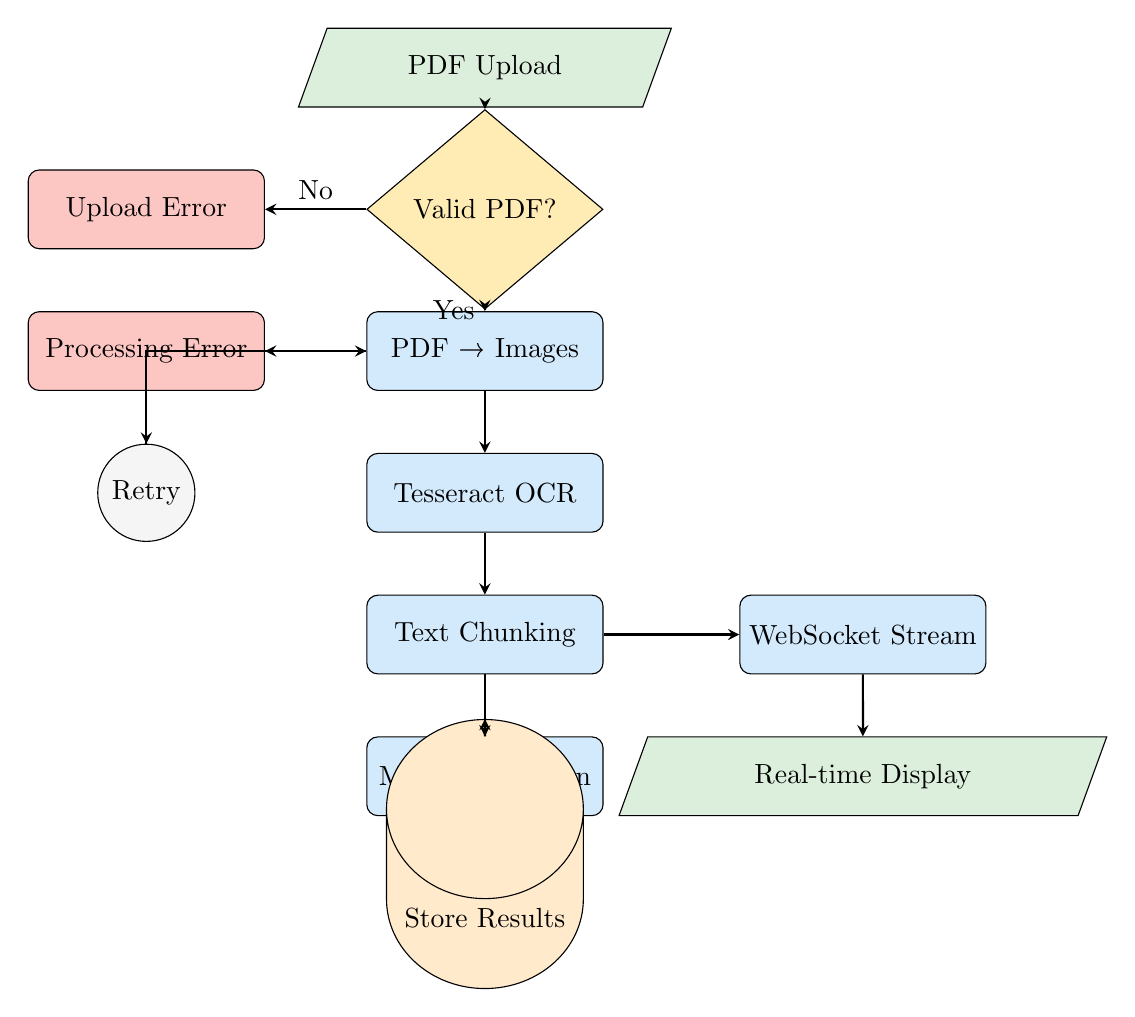
\begin{tikzpicture}[node distance=1.8cm]

% Input Stage
\node (upload) [io] {PDF Upload};
\node (validate) [decision, below of=upload] {Valid PDF?};
\node (error1) [process, left of=validate, xshift=-2.5cm, fill=dangerred!30] {Upload Error};

% Processing Stage
\node (convert) [process, below of=validate] {PDF → Images};
\node (ocr) [process, below of=convert] {Tesseract OCR};
\node (chunk) [process, below of=ocr] {Text Chunking};

% Classification Stage
\node (classify) [process, below of=chunk] {ML Classification};
\node (results) [storage, below of=classify] {Store Results};

% Output Stage
\node (websocket) [process, right of=chunk, xshift=3cm] {WebSocket Stream};
\node (display) [io, below of=websocket] {Real-time Display};

% Error handling
\node (error2) [process, left of=convert, xshift=-2.5cm, fill=dangerred!30] {Processing Error};
\node (retry) [connector, below of=error2] {Retry};

% Arrows
\draw [arrow] (upload) -- (validate);
\draw [arrow] (validate) -- node[anchor=east] {Yes} (convert);
\draw [arrow] (validate) -- node[anchor=south] {No} (error1);
\draw [arrow] (convert) -- (ocr);
\draw [arrow] (ocr) -- (chunk);
\draw [arrow] (chunk) -- (classify);
\draw [arrow] (classify) -- (results);
\draw [arrow] (chunk) -- (websocket);
\draw [arrow] (websocket) -- (display);

% Error flows
\draw [arrow] (convert) -- (error2);
\draw [arrow] (error2) -- (retry);
\draw [arrow] (retry) |- (convert);

\end{tikzpicture}
\caption{Document Processing Pipeline}
\label{fig:processing-pipeline}
\end{figure}

\section{Machine Learning Classification Workflow}

\subsection{Text Classification Process}

\begin{algorithm}[H]
\caption{AI Content Classification Algorithm}
\begin{algorithmic}[1]
\Procedure{ClassifyText}{$text\_chunk$}
    \State $tokens \gets \text{Tokenize}(text\_chunk)$
    \State $input\_ids \gets \text{EncodeToBERT}(tokens)$
    \State $attention\_mask \gets \text{CreateAttentionMask}(input\_ids)$
    
    \State $logits \gets \text{ModelInference}(input\_ids, attention\_mask)$
    \State $probabilities \gets \text{Softmax}(logits)$
    \State $prediction \gets \text{ArgMax}(probabilities)$
    
    \State $confidence \gets \text{Max}(probabilities)$
    
    \If{$confidence < threshold$}
        \State \Return $\text{UNDETERMINED}$
    \Else
        \State \Return $\text{ClassLabels}[prediction]$
    \EndIf
\EndProcedure
\end{algorithmic}
\end{algorithm}

\subsection{Classification Categories}

\begin{table}[H]
\centering
\begin{tabular}{|c|l|l|c|}
\hline
\textbf{Label} & \textbf{Category} & \textbf{Description} & \textbf{Color Code} \\
\hline
0 & AI-Generated & Pure AI-created content & \textcolor{dangerred}{Red} \\
1 & Humanised & AI content edited by humans & \textcolor{accentorange}{Orange} \\
2 & Human-Written & Original human content & \textcolor{secondarygreen}{Green} \\
3 & Polished & Human content with AI assistance & \textcolor{primaryblue}{Blue} \\
4 & Undetermined & Cannot classify with confidence & \textcolor{violet}{Purple} \\
\hline
\end{tabular}
\caption{Content Classification Schema}
\label{tab:classification}
\end{table}

\section{Real-time Communication Flow}

\subsection{WebSocket Data Flow}

\begin{figure}[H]
\centering
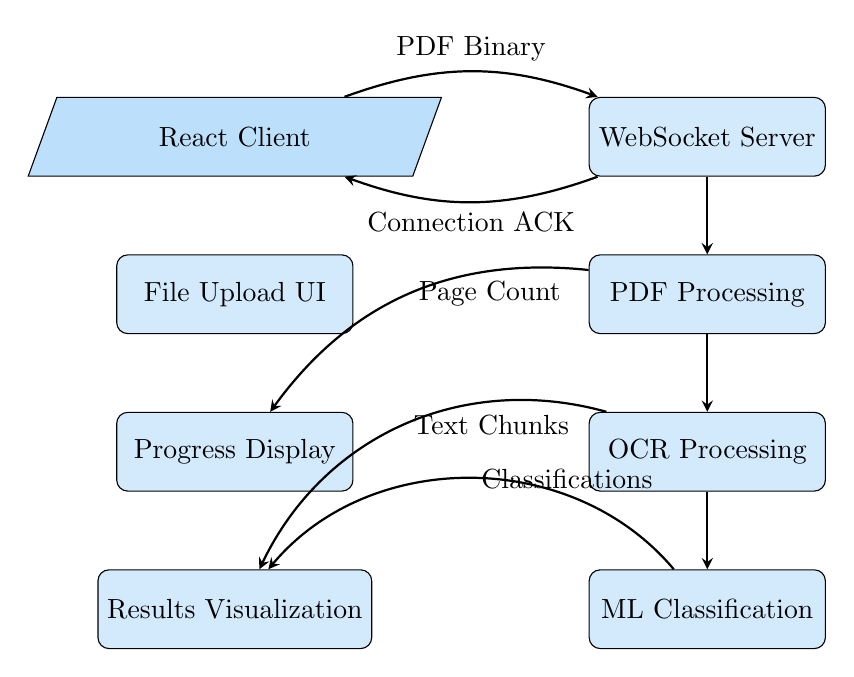
\begin{tikzpicture}[node distance=2cm]

% Client side
\node (client) [io, fill=primaryblue!30] {React Client};
\node (upload_ui) [process, below of=client] {File Upload UI};
\node (progress) [process, below of=upload_ui] {Progress Display};
\node (results) [process, below of=progress] {Results Visualization};

% Server side
\node (websocket) [process, right of=client, xshift=4cm] {WebSocket Server};
\node (pdf_proc) [process, below of=websocket] {PDF Processing};
\node (ocr_proc) [process, below of=pdf_proc] {OCR Processing};
\node (ml_proc) [process, below of=ocr_proc] {ML Classification};

% Data flow arrows
\draw [arrow, bend left=20] (client) to node[above] {PDF Binary} (websocket);
\draw [arrow, bend left=20] (websocket) to node[below] {Connection ACK} (client);

\draw [arrow] (websocket) -- (pdf_proc);
\draw [arrow] (pdf_proc) -- (ocr_proc);
\draw [arrow] (ocr_proc) -- (ml_proc);

\draw [arrow, bend right=30] (pdf_proc) to node[right] {Page Count} (progress);
\draw [arrow, bend right=40] (ocr_proc) to node[right] {Text Chunks} (results);
\draw [arrow, bend right=50] (ml_proc) to node[right] {Classifications} (results);

\end{tikzpicture}
\caption{WebSocket Communication Flow}
\label{fig:websocket-flow}
\end{figure}

\subsection{Message Format Specification}

\begin{tcolorbox}[colback=lightgray, colframe=darkgray, title=WebSocket Message Schema]
\begin{lstlisting}[language=JSON]
{
  "type": "chunk_result",
  "page": 1,
  "chunk": 15,
  "text": "Sample text content for analysis",
  "data": {
    "input": "Sample text content for analysis",
    "result": 2,
    "confidence": 0.87
  },
  "timestamp": "2025-11-05T10:30:00Z"
}
\end{lstlisting}
\end{tcolorbox}

\section{Error Handling and Recovery}

\subsection{Error Classification Matrix}

\begin{table}[H]
\centering
\small
\begin{tabular}{|l|l|l|l|}
\hline
\textbf{Error Type} & \textbf{Severity} & \textbf{Recovery Action} & \textbf{User Notification} \\
\hline
Invalid PDF & Low & Reject upload & "Please select a valid PDF" \\
OCR Failure & Medium & Retry processing & "Processing error, retrying..." \\
ML Model Timeout & Medium & Skip classification & "Classification unavailable" \\
WebSocket Disconnect & High & Reconnect attempt & "Connection lost, reconnecting" \\
Authentication Failure & Critical & Redirect to login & "Please sign in again" \\
\hline
\end{tabular}
\caption{Error Handling Strategy}
\label{tab:error-handling}
\end{table}

\subsection{Fault Tolerance Workflow}

\begin{figure}[H]
\centering
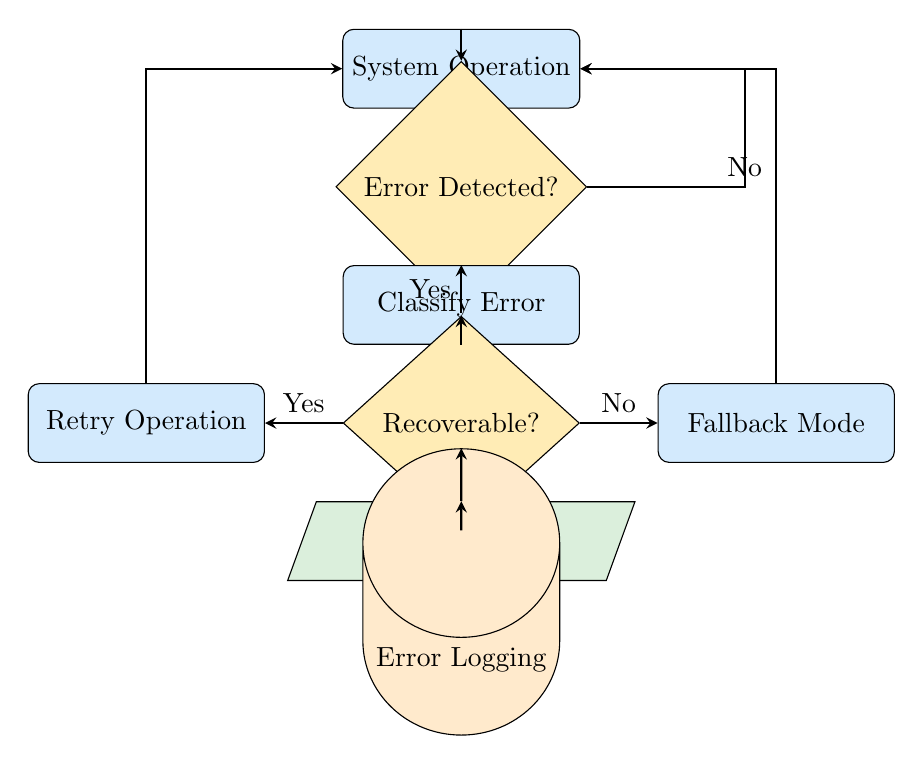
\begin{tikzpicture}[node distance=1.5cm]

\node (operation) [process] {System Operation};
\node (monitor) [decision, below of=operation] {Error Detected?};
\node (classify) [process, below of=monitor] {Classify Error};
\node (recoverable) [decision, below of=classify] {Recoverable?};
\node (retry) [process, left of=recoverable, xshift=-2.5cm] {Retry Operation};
\node (fallback) [process, right of=recoverable, xshift=2.5cm] {Fallback Mode};
\node (notify) [io, below of=recoverable] {Notify User};
\node (log) [storage, below of=notify] {Error Logging};

% Arrows
\draw [arrow] (operation) -- (monitor);
\draw [arrow] (monitor) -- node[anchor=east] {Yes} (classify);
\draw [arrow] (monitor.east) -| node[anchor=south] {No} ++(2,0) |- (operation.east);
\draw [arrow] (classify) -- (recoverable);
\draw [arrow] (recoverable) -- node[anchor=south] {Yes} (retry);
\draw [arrow] (recoverable) -- node[anchor=south] {No} (fallback);
\draw [arrow] (recoverable) -- (notify);
\draw [arrow] (notify) -- (log);
\draw [arrow] (retry) |- (operation);
\draw [arrow] (fallback) |- (operation);

\end{tikzpicture}
\caption{Error Recovery Workflow}
\label{fig:error-recovery}
\end{figure}

\section{Performance Optimization}

\subsection{Processing Performance Metrics}

\begin{table}[H]
\centering
\begin{tabular}{|l|c|c|c|}
\hline
\textbf{Operation} & \textbf{Target Time} & \textbf{Memory Usage} & \textbf{CPU Usage} \\
\hline
PDF Upload & < 2s & 50MB & 10\% \\
PDF to Images & < 5s/page & 100MB/page & 30\% \\
OCR Processing & < 3s/page & 200MB/page & 50\% \\
ML Classification & < 0.5s/chunk & 1GB & 80\% \\
Result Display & < 0.1s & 10MB & 5\% \\
\hline
\end{tabular}
\caption{Performance Benchmarks}
\label{tab:performance}
\end{table}

\subsection{Optimization Strategies}

\begin{itemize}
    \item \textbf{Chunked Processing}: Process documents in parallel chunks
    \item \textbf{Caching}: Cache OCR results and model predictions
    \item \textbf{Lazy Loading}: Load model weights on demand
    \item \textbf{Connection Pooling}: Reuse WebSocket connections
    \item \textbf{Compression}: Compress large data transfers
    \item \textbf{Progressive Rendering}: Display results as they arrive
\end{itemize}

\section{Security Architecture}

\subsection{Security Layers}

\begin{figure}[H]
\centering
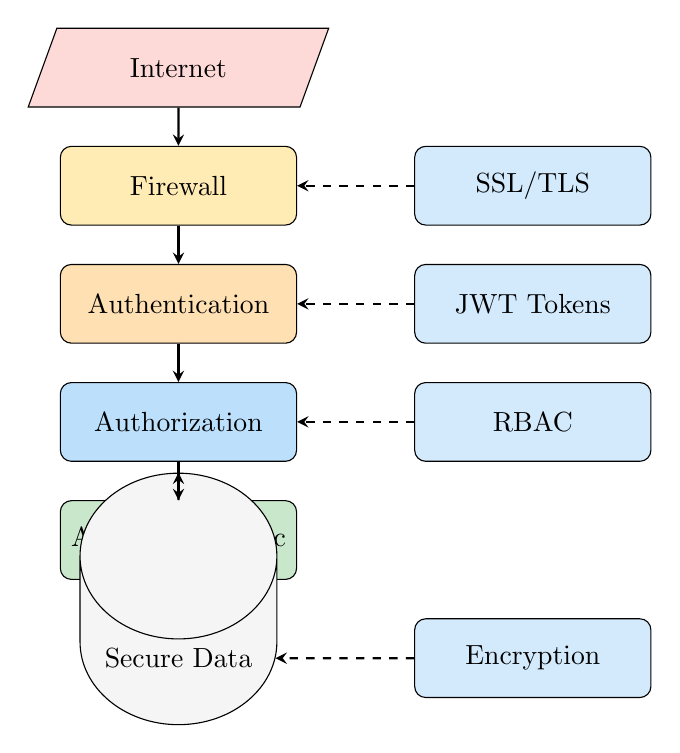
\begin{tikzpicture}[node distance=1.5cm]

% Security layers from outside to inside
\node (internet) [io, fill=dangerred!20] {Internet};
\node (firewall) [process, below of=internet, fill=warningyellow!30] {Firewall};
\node (auth) [process, below of=firewall, fill=accentorange!30] {Authentication};
\node (authorization) [process, below of=auth, fill=primaryblue!30] {Authorization};
\node (application) [process, below of=authorization, fill=secondarygreen!30] {Application Logic};
\node (data) [storage, below of=application, fill=lightgray] {Secure Data};

% Security annotations
\node (ssl) [process, right of=firewall, xshift=3cm, fill=primaryblue!20] {SSL/TLS};
\node (jwt) [process, right of=auth, xshift=3cm, fill=primaryblue!20] {JWT Tokens};
\node (rbac) [process, right of=authorization, xshift=3cm, fill=primaryblue!20] {RBAC};
\node (encryption) [process, right of=data, xshift=3cm, fill=primaryblue!20] {Encryption};

% Arrows
\draw [arrow] (internet) -- (firewall);
\draw [arrow] (firewall) -- (auth);
\draw [arrow] (auth) -- (authorization);
\draw [arrow] (authorization) -- (application);
\draw [arrow] (application) -- (data);

% Security feature arrows
\draw [arrow, dashed] (ssl) -- (firewall);
\draw [arrow, dashed] (jwt) -- (auth);
\draw [arrow, dashed] (rbac) -- (authorization);
\draw [arrow, dashed] (encryption) -- (data);

\end{tikzpicture}
\caption{Security Architecture Layers}
\label{fig:security-layers}
\end{figure}

\section{Monitoring and Observability}

\subsection{Distributed Tracing Flow}

\begin{figure}[H]
\centering
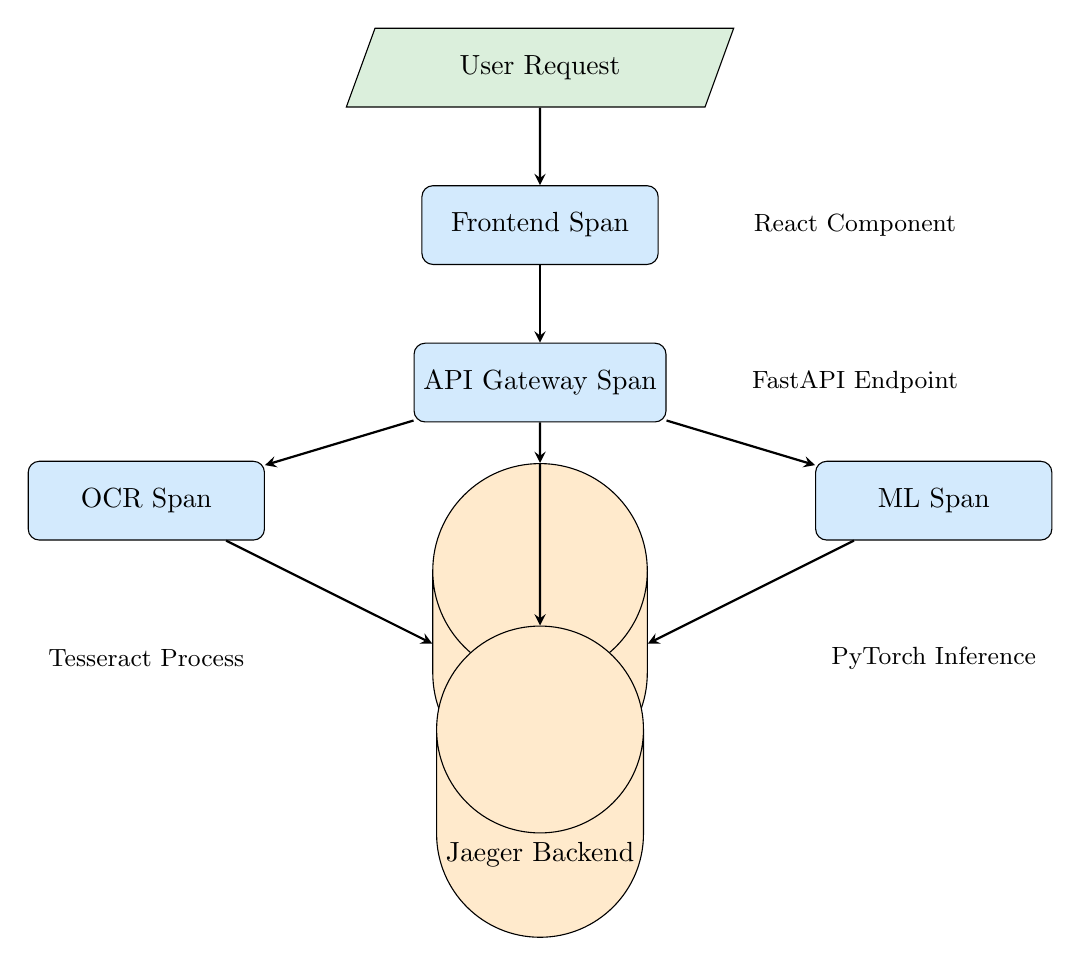
\begin{tikzpicture}[node distance=2cm]

% Request flow with tracing
\node (request) [io] {User Request};
\node (frontend_trace) [process, below of=request] {Frontend Span};
\node (api_trace) [process, below of=frontend_trace] {API Gateway Span};
\node (ocr_trace) [process, left of=api_trace, xshift=-3cm, yshift=-1.5cm] {OCR Span};
\node (ml_trace) [process, right of=api_trace, xshift=3cm, yshift=-1.5cm] {ML Span};
\node (collector) [storage, below of=api_trace, yshift=-2cm] {OTEL Collector};
\node (jaeger) [storage, below of=collector] {Jaeger Backend};

% Trace relationships
\draw [arrow] (request) -- (frontend_trace);
\draw [arrow] (frontend_trace) -- (api_trace);
\draw [arrow] (api_trace) -- (ocr_trace);
\draw [arrow] (api_trace) -- (ml_trace);
\draw [arrow] (ocr_trace) -- (collector);
\draw [arrow] (ml_trace) -- (collector);
\draw [arrow] (api_trace) -- (collector);
\draw [arrow] (collector) -- (jaeger);

% Span annotations
\node [right of=frontend_trace, xshift=2cm] {\small React Component};
\node [right of=api_trace, xshift=2cm] {\small FastAPI Endpoint};
\node [below of=ocr_trace] {\small Tesseract Process};
\node [below of=ml_trace] {\small PyTorch Inference};

\end{tikzpicture}
\caption{Distributed Tracing Architecture}
\label{fig:tracing-flow}
\end{figure}

\section{Deployment Architecture}

\subsection{Production Deployment Flow}

\begin{figure}[H]
\centering
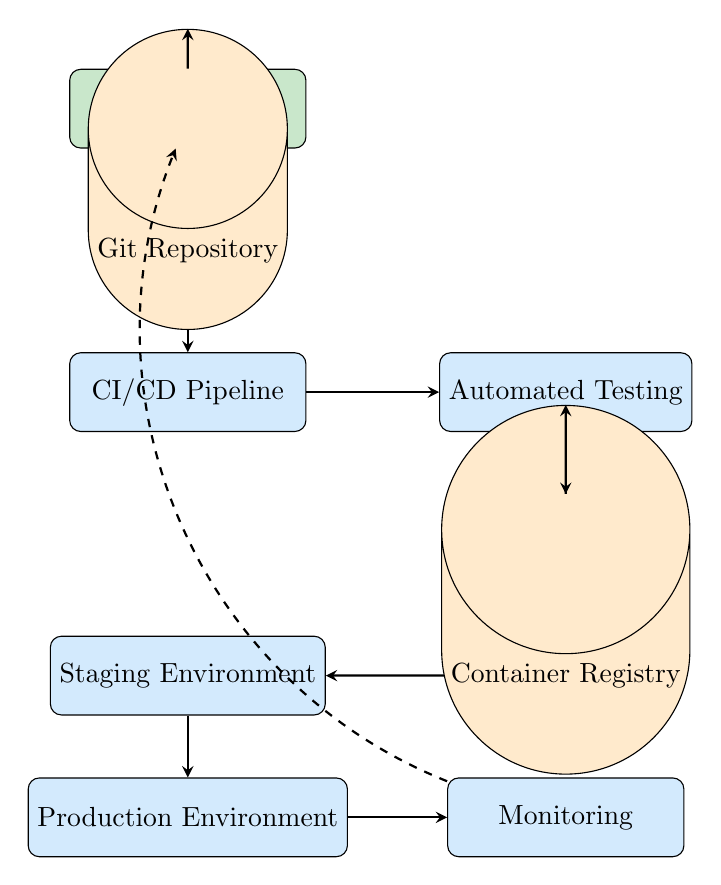
\begin{tikzpicture}[node distance=1.8cm]

% Development
\node (dev) [process, fill=secondarygreen!30] {Development};
\node (git) [storage, below of=dev] {Git Repository};
\node (ci) [process, below of=git] {CI/CD Pipeline};

% Testing
\node (test) [process, right of=ci, xshift=3cm] {Automated Testing};
\node (build) [process, below of=test] {Docker Build};
\node (registry) [storage, below of=build] {Container Registry};

% Deployment
\node (staging) [process, left of=registry, xshift=-3cm] {Staging Environment};
\node (prod) [process, below of=staging] {Production Environment};
\node (monitor) [process, right of=prod, xshift=3cm] {Monitoring};

% Arrows
\draw [arrow] (dev) -- (git);
\draw [arrow] (git) -- (ci);
\draw [arrow] (ci) -- (test);
\draw [arrow] (test) -- (build);
\draw [arrow] (build) -- (registry);
\draw [arrow] (registry) -- (staging);
\draw [arrow] (staging) -- (prod);
\draw [arrow] (prod) -- (monitor);

% Feedback loop
\draw [arrow, dashed, bend left=45] (monitor) to (dev);

\end{tikzpicture}
\caption{Deployment Pipeline}
\label{fig:deployment-pipeline}
\end{figure}

\section{Future Enhancements}

\subsection{Planned Features}
\begin{enumerate}
    \item \textbf{Multi-language Support}: Extend OCR and classification to multiple languages
    \item \textbf{Batch Processing}: Support for multiple document analysis
    \item \textbf{Advanced Analytics}: Statistical analysis and reporting dashboard
    \item \textbf{API Integration}: RESTful API for third-party integrations
    \item \textbf{Mobile Application}: Native mobile app for document scanning
    \item \textbf{Cloud Deployment}: Kubernetes-based cloud infrastructure
\end{enumerate}

\subsection{Scalability Considerations}
\begin{itemize}
    \item \textbf{Horizontal Scaling}: Load balancing across multiple instances
    \item \textbf{Database Optimization}: Implement caching layers and read replicas
    \item \textbf{CDN Integration}: Content delivery network for static assets
    \item \textbf{Microservices}: Decompose monolithic components into microservices
    \item \textbf{Queue Management}: Implement message queues for async processing
\end{itemize}

\section{Conclusion}

The \systemname{} represents a comprehensive solution for AI content detection in documents, combining state-of-the-art machine learning techniques with modern web technologies. The system's modular architecture ensures scalability, maintainability, and extensibility for future enhancements. The real-time processing capabilities and intuitive user interface make it an effective tool for academic and research applications.

The workflow documentation presented here provides a complete technical overview of the system's operation, from user authentication through document processing to result visualization. This architecture supports the system's goals of accuracy, performance, and user experience while maintaining security and observability standards.

\section*{References}

\begin{enumerate}
    \item FastAPI Documentation: \url{https://fastapi.tiangolo.com/}
    \item React Documentation: \url{https://reactjs.org/docs/}
    \item OpenTelemetry Specification: \url{https://opentelemetry.io/docs/}
    \item Tesseract OCR Documentation: \url{https://tesseract-ocr.github.io/}
    \item PyTorch Documentation: \url{https://pytorch.org/docs/}
    \item Material-UI Component Library: \url{https://mui.com/}
\end{enumerate}

\end{document}
